% ============================================================================
% PromptSeg-Lite: Internship Report — Origin AI
% Author: Chidwipak K
% Compile: pdflatex internship_report.tex (×2 for references)
% ============================================================================
\documentclass[12pt,a4paper]{article}

% ---------- packages --------------------------------------------------------
\usepackage[utf8]{inputenc}
\usepackage[T1]{fontenc}
\usepackage{lmodern}
\usepackage[margin=2.5cm]{geometry}
\usepackage{graphicx}
\usepackage{booktabs}
\usepackage{array}
\usepackage{hyperref}
\usepackage{xcolor}
\usepackage{amsmath,amssymb}
\usepackage{float}
\usepackage{caption}
\usepackage{subcaption}
\usepackage{enumitem}
\usepackage{fancyhdr}
\usepackage{titlesec}
\usepackage{tcolorbox}
\usepackage{multirow}
\usepackage{tabularx}
\usepackage{setspace}

% ---------- style -----------------------------------------------------------
\hypersetup{
  colorlinks=true,
  linkcolor=blue!60!black,
  urlcolor=blue!70!black,
  citecolor=blue!50!black,
}

\definecolor{originblue}{HTML}{1a73e8}
\definecolor{boxbg}{HTML}{f0f7ff}

\pagestyle{fancy}
\fancyhf{}
\fancyhead[L]{\small PromptSeg-Lite --- Internship Report}
\fancyhead[R]{\small Chidwipak K}
\fancyfoot[C]{\thepage}
\renewcommand{\headrulewidth}{0.4pt}

\titleformat{\section}{\Large\bfseries\color{originblue}}{\thesection}{1em}{}
\titleformat{\subsection}{\large\bfseries}{\thesubsection}{1em}{}

\setlength{\parskip}{0.6em}
\setlength{\parindent}{0pt}
\onehalfspacing

% ---------- document --------------------------------------------------------
\begin{document}

% ===== TITLE PAGE ===========================================================
\begin{titlepage}
\centering
\vspace*{2cm}
{\Huge\bfseries\color{originblue} PromptSeg-Lite\\[0.3em]}
{\LARGE Prompted Segmentation for Drywall QA\\[2em]}
{\Large Internship Report --- Origin AI\\[1.5em]}
\rule{0.6\textwidth}{0.5pt}\\[2em]
{\large\textbf{Author:} Chidwipak K\\[0.5em]}
{\large\textbf{Date:} April 2026\\[0.5em]}
{\large\textbf{Hardware:} NVIDIA L4 GPU (24\,GB), GCP\\[3em]}
\vfill
{\small Built entirely from scratch --- no pretrained weights.}
\end{titlepage}

% ===== TABLE OF CONTENTS ====================================================
\tableofcontents
\newpage

% ===== 1. GOAL SUMMARY ======================================================
\section{Goal Summary}

The objective was to build a \textbf{text-prompted binary segmentation model from scratch} that can detect two categories of drywall damage---\emph{taping areas} and \emph{surface cracks}---by conditioning on a natural-language prompt such as \texttt{"segment crack"} or \texttt{"segment taping area"}.

I designed \textbf{PromptSeg-Lite}, a lightweight U-Net with a character-level BiLSTM text encoder and Feature-wise Linear Modulation (FiLM).  The model takes an RGB image and a text prompt, and produces a pixel-level binary mask.  I trained everything from scratch on an NVIDIA L4 GPU with no pretrained backbone.

\begin{tcolorbox}[colback=boxbg, colframe=originblue, title=Key Results]
\begin{itemize}[nosep]
  \item \textbf{V1 Baseline:} mIoU = 0.7019, Dice = 0.7662 (256$\times$256, 2.08\,M params)
  \item \textbf{V2 Final:}   mIoU = 0.7300, Dice = 0.7796 (512$\times$512, 2.75\,M params)
  \item \textbf{Inference:}   9.7\,ms/image (103 FPS) on NVIDIA L4
  \item \textbf{Model size:}  11.01\,MB (FP32)
\end{itemize}
\end{tcolorbox}

% ===== 2. LIVE DEMO & REPOSITORY ============================================
\section{Live Demo \& Repository}

\begin{tcolorbox}[colback=boxbg, colframe=originblue, title=Links]
\begin{itemize}[nosep]
  \item \textbf{Streamlit App:} \url{https://promptseg-lite.streamlit.app}
        \hfill\textit{(upload any wall image, pick a prompt, see the mask)}
  \item \textbf{GitHub Repo:} \url{https://github.com/chidwipak/PromptSeg-Lite}
\end{itemize}
\end{tcolorbox}

The Streamlit demo supports both V1 and V2 checkpoints, six built-in prompts, custom text input, and a prompt-comparison mode that segments the same image with two different prompts side by side.

% ===== 3. APPROACH & ARCHITECTURE ===========================================
\section{Approach \& Architecture: The V1~$\to$~V2 Journey}

\subsection{V1 Baseline}

I started with a straightforward design:

\begin{itemize}[nosep]
  \item \textbf{Encoder:} four-stage depthwise-separable CNN (channels 64$\to$128$\to$256$\to$512) with Squeeze-and-Excitation attention after each stage.
  \item \textbf{Text encoder:} character-level BiLSTM (vocab 128, embed 64, hidden 128$\times$2).
  \item \textbf{Conditioning:} FiLM layers inject text information at every encoder and decoder stage (7 FiLM generators total).
  \item \textbf{Decoder:} symmetric U-Net decoder with skip connections.
  \item \textbf{Loss:} Dice + BCE (equal weight).
  \item \textbf{Resolution:} 256$\times$256.
\end{itemize}

V1 reached \textbf{mIoU = 0.7019} in 150 epochs ($\sim$40 min).  Taping segmentation was solid (IoU 0.80), but thin cracks were the bottleneck (IoU 0.60).  I noticed two problems: fine cracks at 256$\times$256 were sub-pixel, and the equal-weight loss did not punish missed crack pixels enough.

\subsection{V2 Upgrades}

To address V1's weaknesses, I made five targeted changes:

\begin{enumerate}[nosep]
  \item \textbf{512$\times$512 resolution} --- 4$\times$ more pixels make thin cracks visible.
  \item \textbf{ASPP bottleneck} --- Atrous Spatial Pyramid Pooling at dilation rates 6, 12, 18 captures multi-scale context (five parallel branches fused into 512 channels).
  \item \textbf{Focal Tversky Loss} ($\alpha$=0.7, $\beta$=0.3, $\gamma$=0.75) --- penalises false negatives (missed cracks) far more than false positives.
  \item \textbf{Boundary Loss} (5$\times$ weight on morphological boundaries) + \textbf{OHEM} (top 25\% hardest pixels) --- focuses learning on crack edges and ambiguous regions.
  \item \textbf{Deep Supervision} --- auxiliary heads at $\frac{1}{32}$ and $\frac{1}{16}$ resolution with weights 0.4 and 0.2 stabilise early training at the higher resolution.
\end{enumerate}

V2 reached \textbf{mIoU = 0.7300} in 200 epochs ($\sim$1.5 h), a +2.81 percentage-point improvement.

\subsection{Architecture Diagram}

Figure~\ref{fig:arch} shows the full V2 pipeline.

\begin{figure}[H]
\centering
\fbox{\parbox{0.9\textwidth}{\centering\vspace{2em}
\textit{Architecture diagram placeholder.}\\
Text Prompt $\to$ BiLSTM $\to$ FiLM $\to$ Encoder (4 stages) $\to$ ASPP $\to$ Decoder (4 stages) $\to$ Mask\\
Skip connections link encoder stages to corresponding decoder stages.
\vspace{2em}}}
\caption{PromptSeg-Lite V2 architecture overview.}
\label{fig:arch}
\end{figure}

% ===== 4. DATA SPLIT & AUGMENTATION =========================================
\section{Data Split \& Augmentation}

\subsection{Dataset Sources}

\begin{table}[H]
\centering
\caption{Datasets used.}
\begin{tabular}{llll}
\toprule
\textbf{Dataset} & \textbf{Source} & \textbf{Prompt Class} & \textbf{Annotation} \\
\midrule
Drywall Taping & Roboflow (objectdetect) & \texttt{segment taping area} & COCO bbox $\to$ filled rect \\
Surface Cracks & Roboflow (hemant-ramphul) & \texttt{segment crack}       & COCO polygon \\
\bottomrule
\end{tabular}
\end{table}

\subsection{Split Counts}

\begin{table}[H]
\centering
\caption{Train / Validation split.}
\begin{tabular}{lrrr}
\toprule
\textbf{Class} & \textbf{Train} & \textbf{Valid} & \textbf{Total} \\
\midrule
Drywall Taping & 820  & 202 & 1\,022 \\
Surface Cracks & 2\,818 & 806 & 3\,624 \\
\midrule
\textbf{Combined} & \textbf{3\,638} & \textbf{1\,008} & \textbf{4\,646} \\
\bottomrule
\end{tabular}
\end{table}

To handle the 1:3.4 class imbalance I used a \textbf{weighted random sampler} --- each epoch draws roughly equal numbers of taping and crack samples.

\subsection{Augmentation Pipeline}

Applied during training only:

\begin{itemize}[nosep]
  \item Random horizontal flip ($p$=0.5), vertical flip ($p$=0.3)
  \item Random rotation ($\pm$15\textdegree)
  \item Colour jitter (brightness 0.4, contrast 0.4, saturation 0.3, hue 0.1)
  \item Gaussian blur ($k$=5, $\sigma$\,=\,0.1--2.0, $p$=0.3)
  \item Gaussian noise ($\sigma$=0.02, $p$=0.2)
  \item ImageNet normalisation
\end{itemize}

% ===== 5. METRICS ============================================================
\section{Metrics: V1 vs V2 Comparison}

\subsection{Evaluation Protocol}

All metrics use a threshold of 0.5 on the predicted probability map.  IoU and Dice are computed per-image and averaged.  mIoU is the mean of per-class IoU values.

\subsection{Quantitative Results}

\begin{table}[H]
\centering
\caption{V1 vs V2 comparison on the validation set.}
\label{tab:v1v2}
\begin{tabular}{lcccc}
\toprule
\textbf{Metric} & \textbf{V1} & \textbf{V2} & \textbf{$\Delta$} & \textbf{Improvement} \\
\midrule
\textbf{mIoU}          & 0.7019 & 0.7300 & +0.0281 & +2.81\,pp \\
\textbf{Dice (Overall)} & 0.7662 & 0.7796 & +0.0134 & +1.34\,pp \\
\midrule
Dice (Taping)  & 0.8800 & 0.9050 & +0.0250 & +2.50\,pp \\
IoU (Taping)   & 0.8040 & 0.8472 & +0.0432 & +4.32\,pp \\
Dice (Crack)   & 0.7377 & 0.7481 & +0.0104 & +1.04\,pp \\
IoU (Crack)    & 0.5999 & 0.6128 & +0.0129 & +1.29\,pp \\
\midrule
Parameters     & 2.08\,M & 2.75\,M & +672\,K & +32\% \\
Model size     & 8.3\,MB & 11.01\,MB & +2.71\,MB & +33\% \\
Inference (ms) & 7.76  & 9.70  & +1.94  & +25\% \\
Throughput     & 129 FPS & 103 FPS & $-$26 & $-$20\% \\
\bottomrule
\end{tabular}
\end{table}

The upgrade improved every segmentation metric while keeping the model under 3\,M parameters.

\subsection{Training Curves}

\begin{figure}[H]
\centering
\begin{subfigure}{0.48\textwidth}
  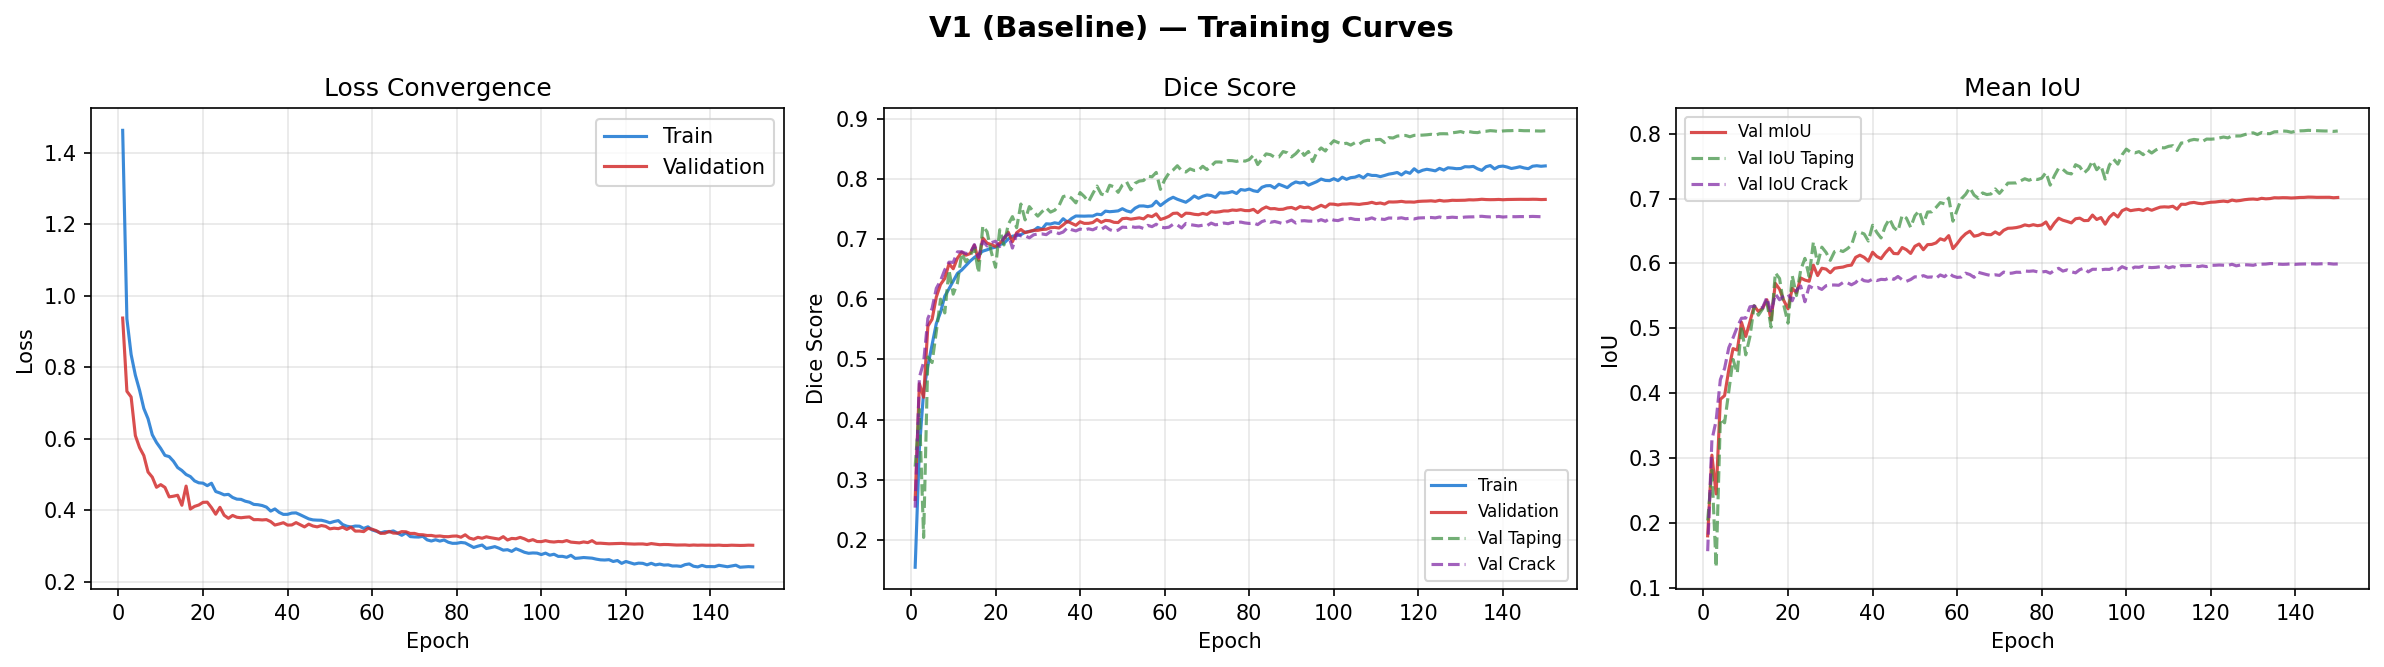
\includegraphics[width=\textwidth]{figures/v1/01_training_curves.png}
  \caption{V1 (150 epochs, best at epoch 146)}
\end{subfigure}
\hfill
\begin{subfigure}{0.48\textwidth}
  
\includegraphics[width=\textwidth]{figures/v2/01_training_curves.png}
  \caption{V2 (200 epochs, best at epoch 191)}
\end{subfigure}
\caption{Training \& validation loss/Dice/mIoU curves.}
\label{fig:training}
\end{figure}

\subsection{Metrics Summary}

\begin{figure}[H]
\centering
\begin{subfigure}{0.48\textwidth}
  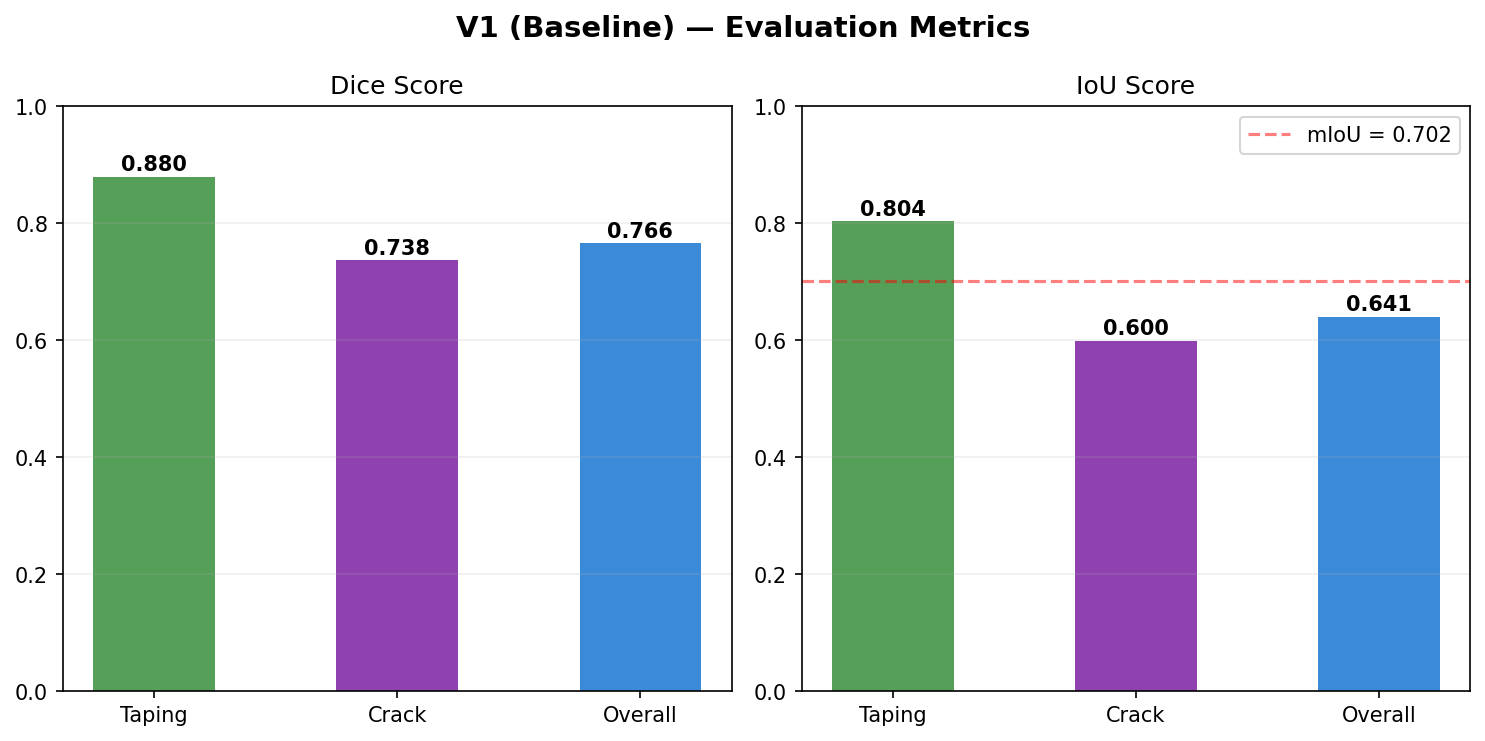
\includegraphics[width=\textwidth]{figures/v1/06_metrics_summary.png}
  \caption{V1 per-class Dice \& IoU}
\end{subfigure}
\hfill
\begin{subfigure}{0.48\textwidth}
  
\includegraphics[width=\textwidth]{figures/v2/06_metrics_summary.png}
  \caption{V2 per-class Dice \& IoU}
\end{subfigure}
\caption{Per-class metric bar charts.}
\label{fig:metrics}
\end{figure}

% ===== 6. VISUAL EXAMPLES ===================================================
\section{Visual Examples}

\subsection{Prediction Quality}

\begin{figure}[H]
\centering
\begin{subfigure}{0.48\textwidth}
  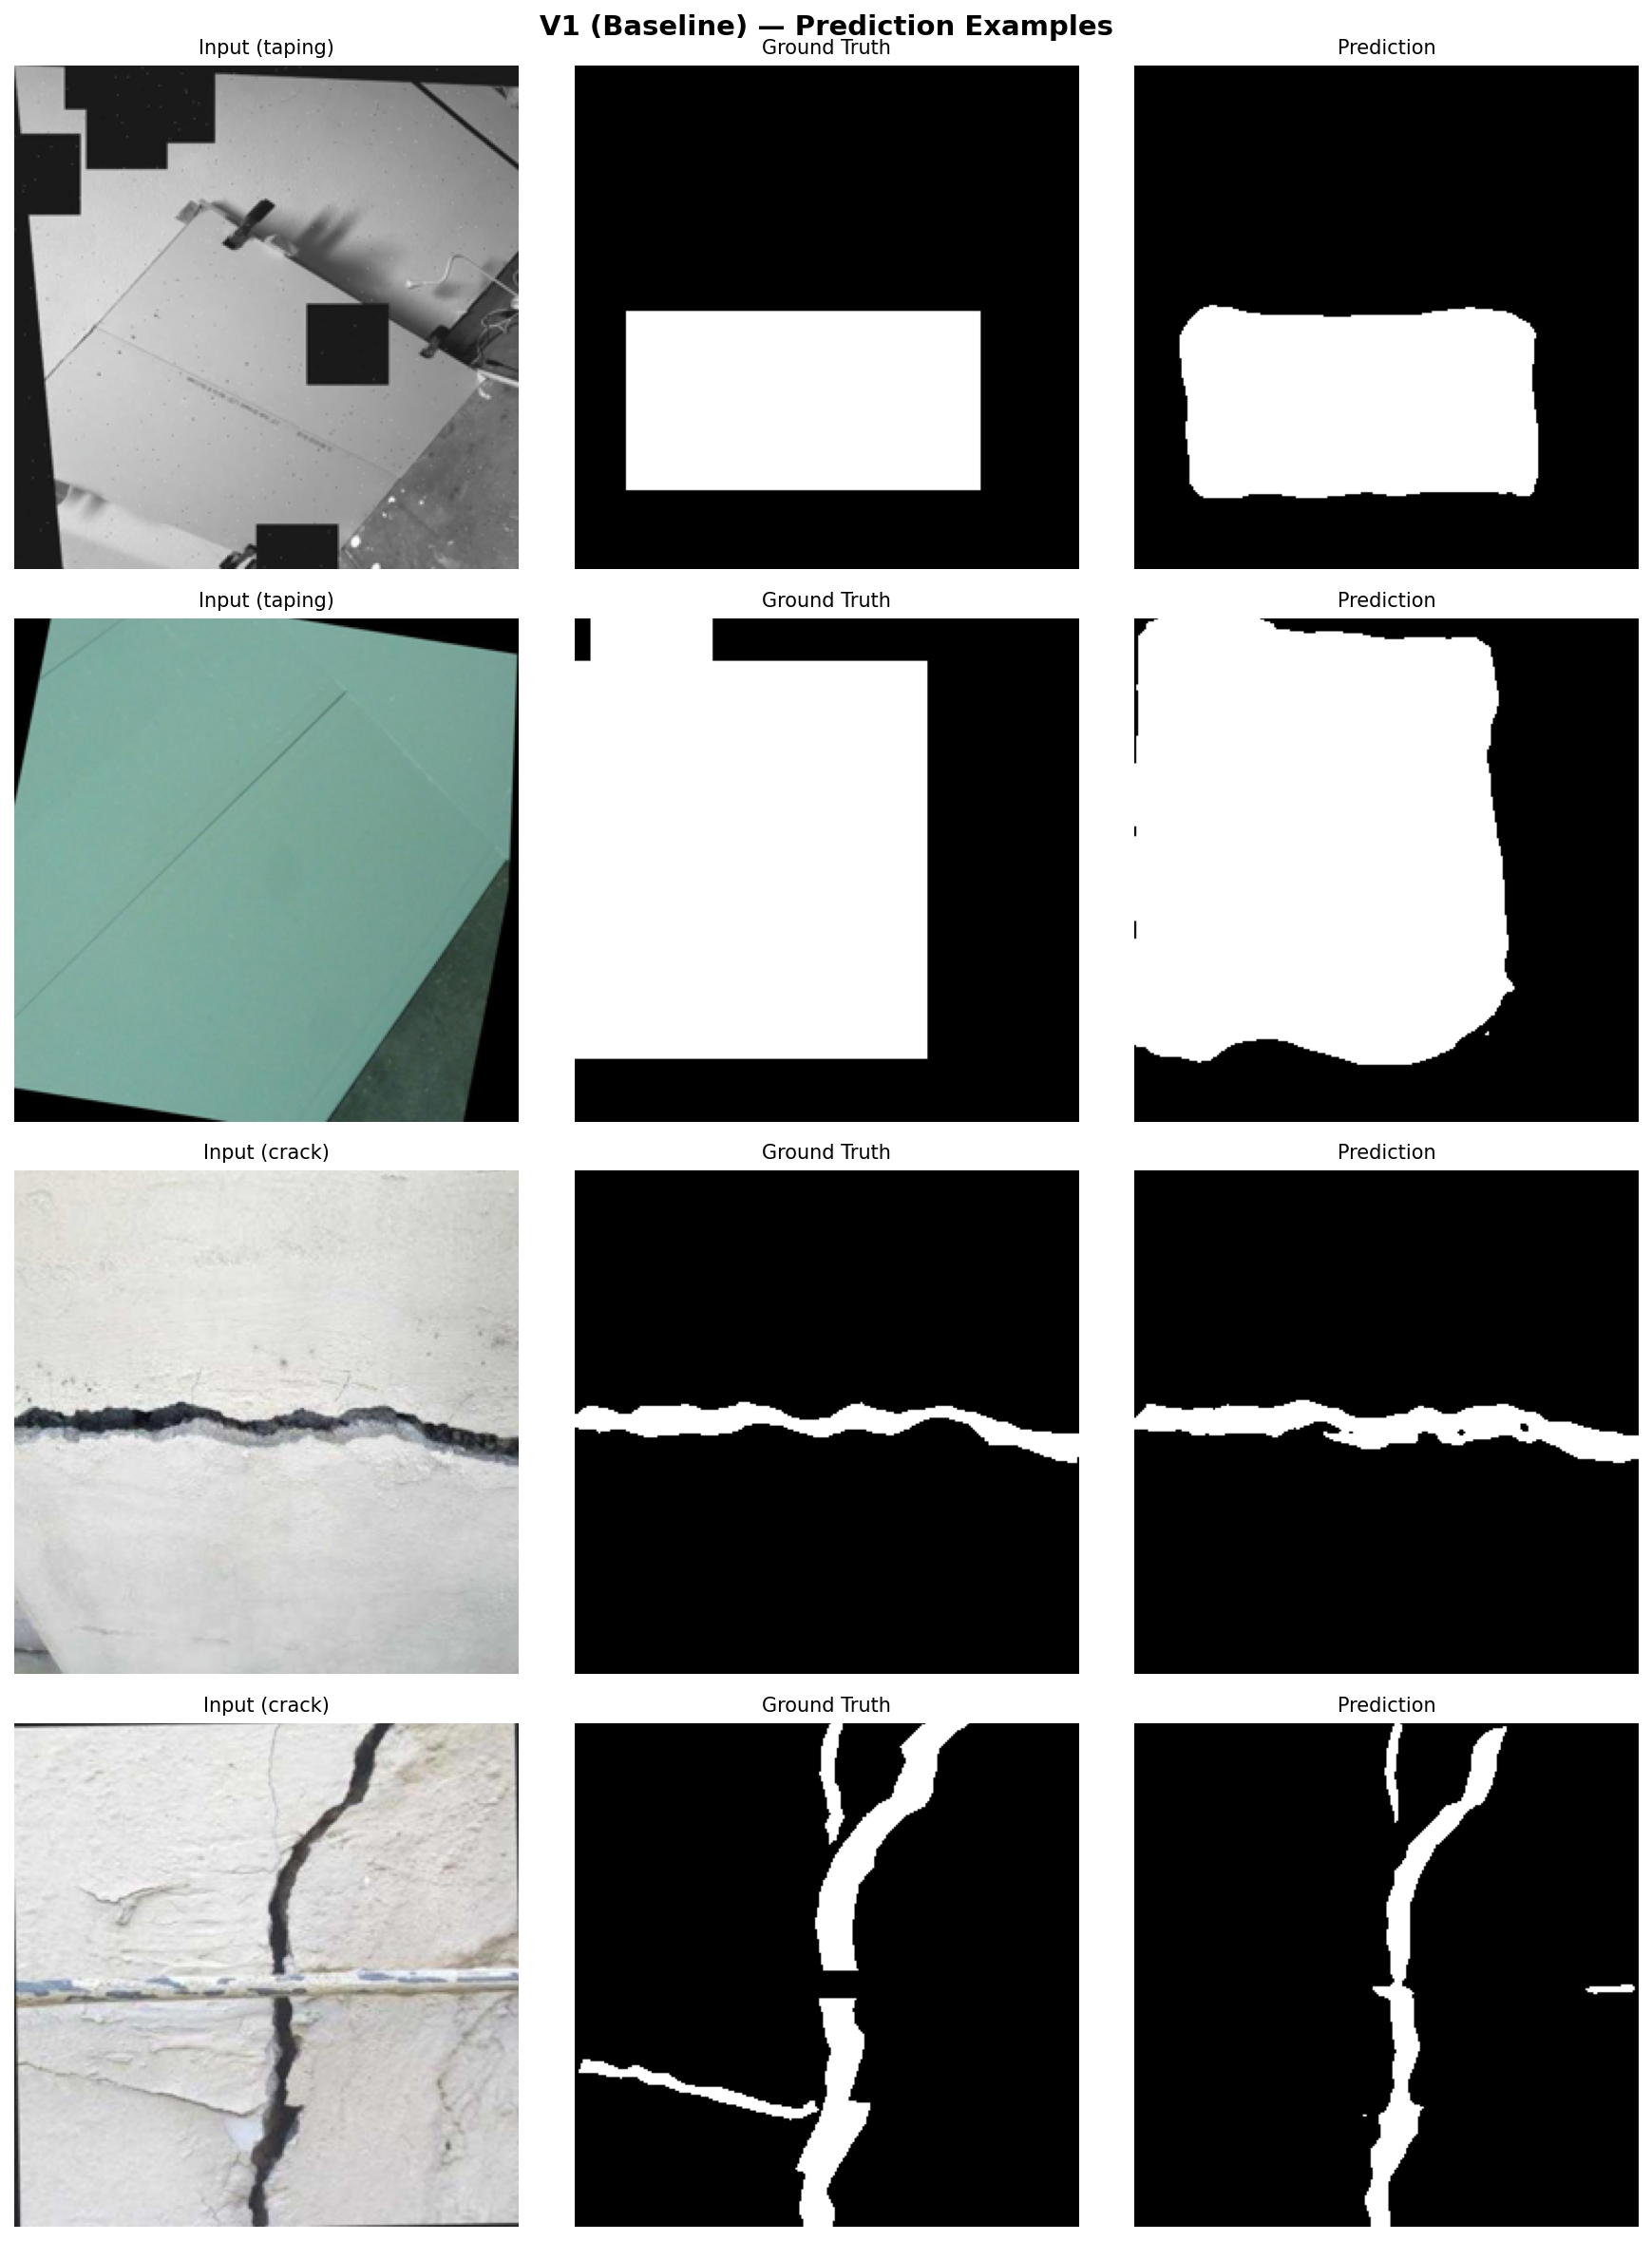
\includegraphics[width=\textwidth]{figures/v1/02_predictions.png}
  \caption{V1 predictions}
\end{subfigure}
\hfill
\begin{subfigure}{0.48\textwidth}
  
\includegraphics[width=\textwidth]{figures/v2/02_predictions.png}
  \caption{V2 predictions}
\end{subfigure}
\caption{Original $|$ Ground Truth $|$ Prediction for selected samples.}
\label{fig:predictions}
\end{figure}

\subsection{Encoder Feature Maps}

\begin{figure}[H]
\centering
\begin{subfigure}{0.48\textwidth}
  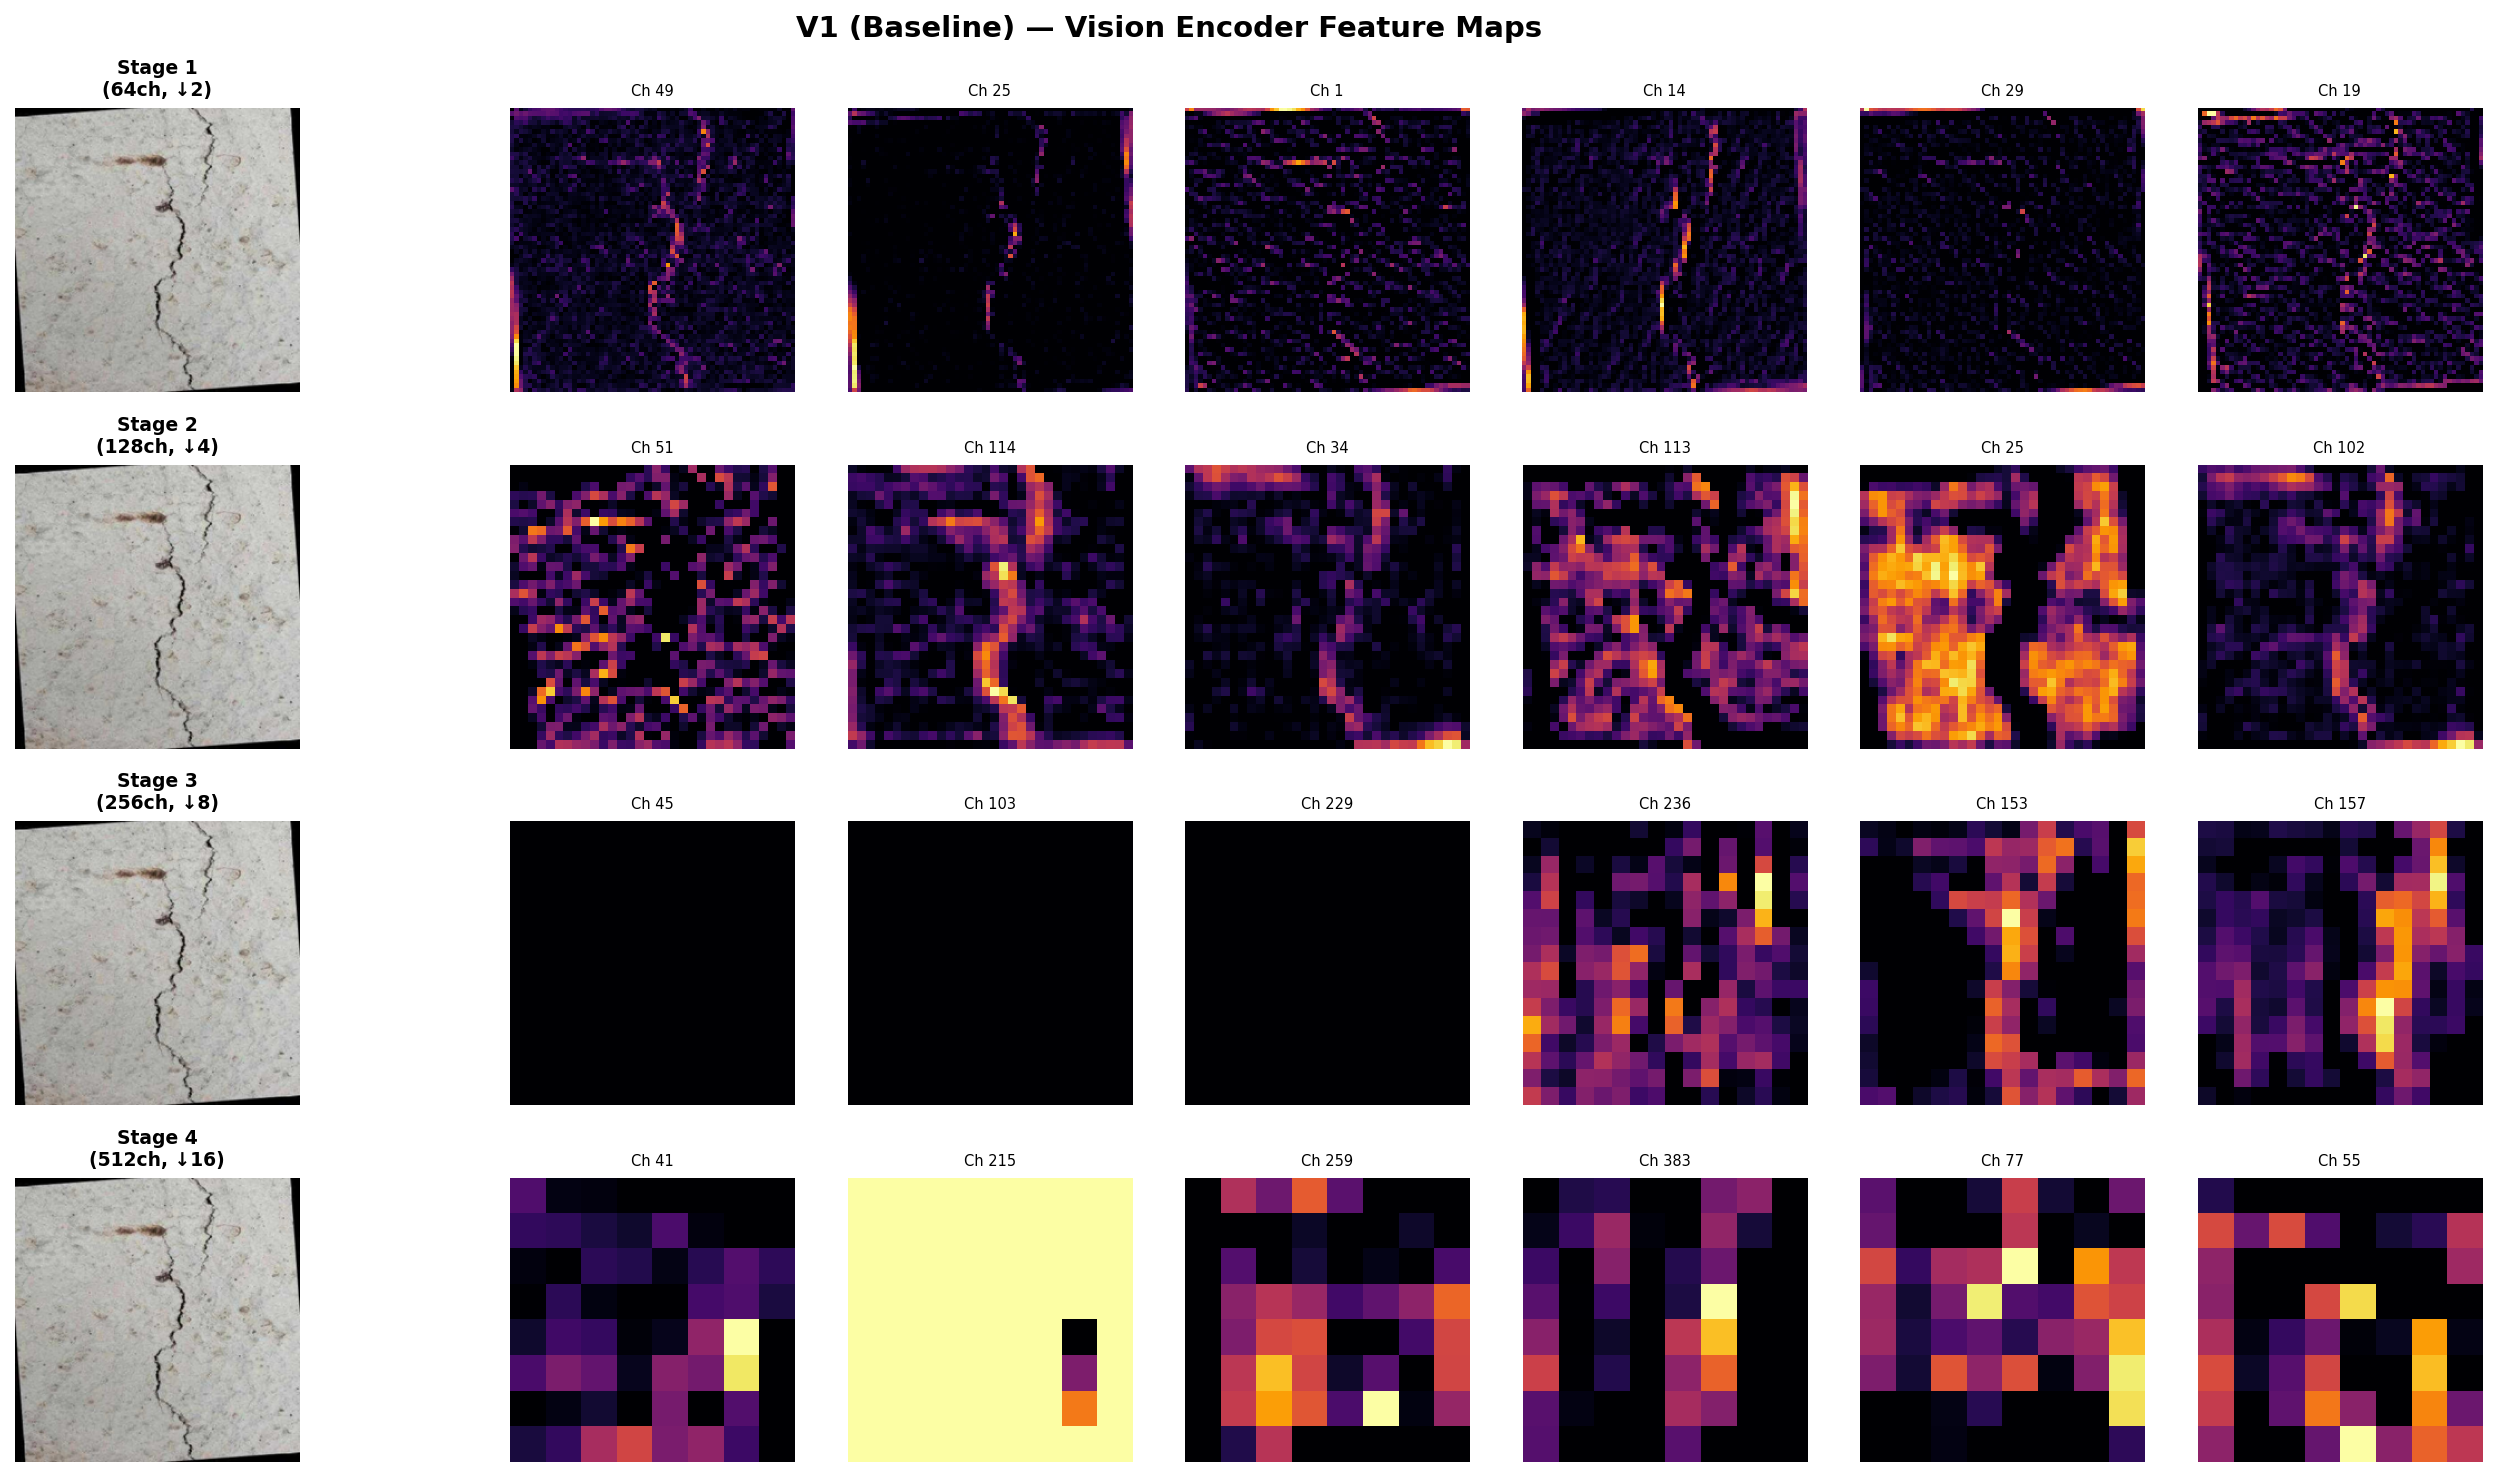
\includegraphics[width=\textwidth]{figures/v1/03_encoder_features.png}
  \caption{V1 encoder activations}
\end{subfigure}
\hfill
\begin{subfigure}{0.48\textwidth}
  
\includegraphics[width=\textwidth]{figures/v2/03_encoder_features.png}
  \caption{V2 encoder activations}
\end{subfigure}
\caption{Learned feature maps across encoder stages (8 channels per stage).}
\label{fig:features}
\end{figure}

\subsection{Text Conditioning (FiLM)}

\begin{figure}[H]
\centering
\begin{subfigure}{0.48\textwidth}
  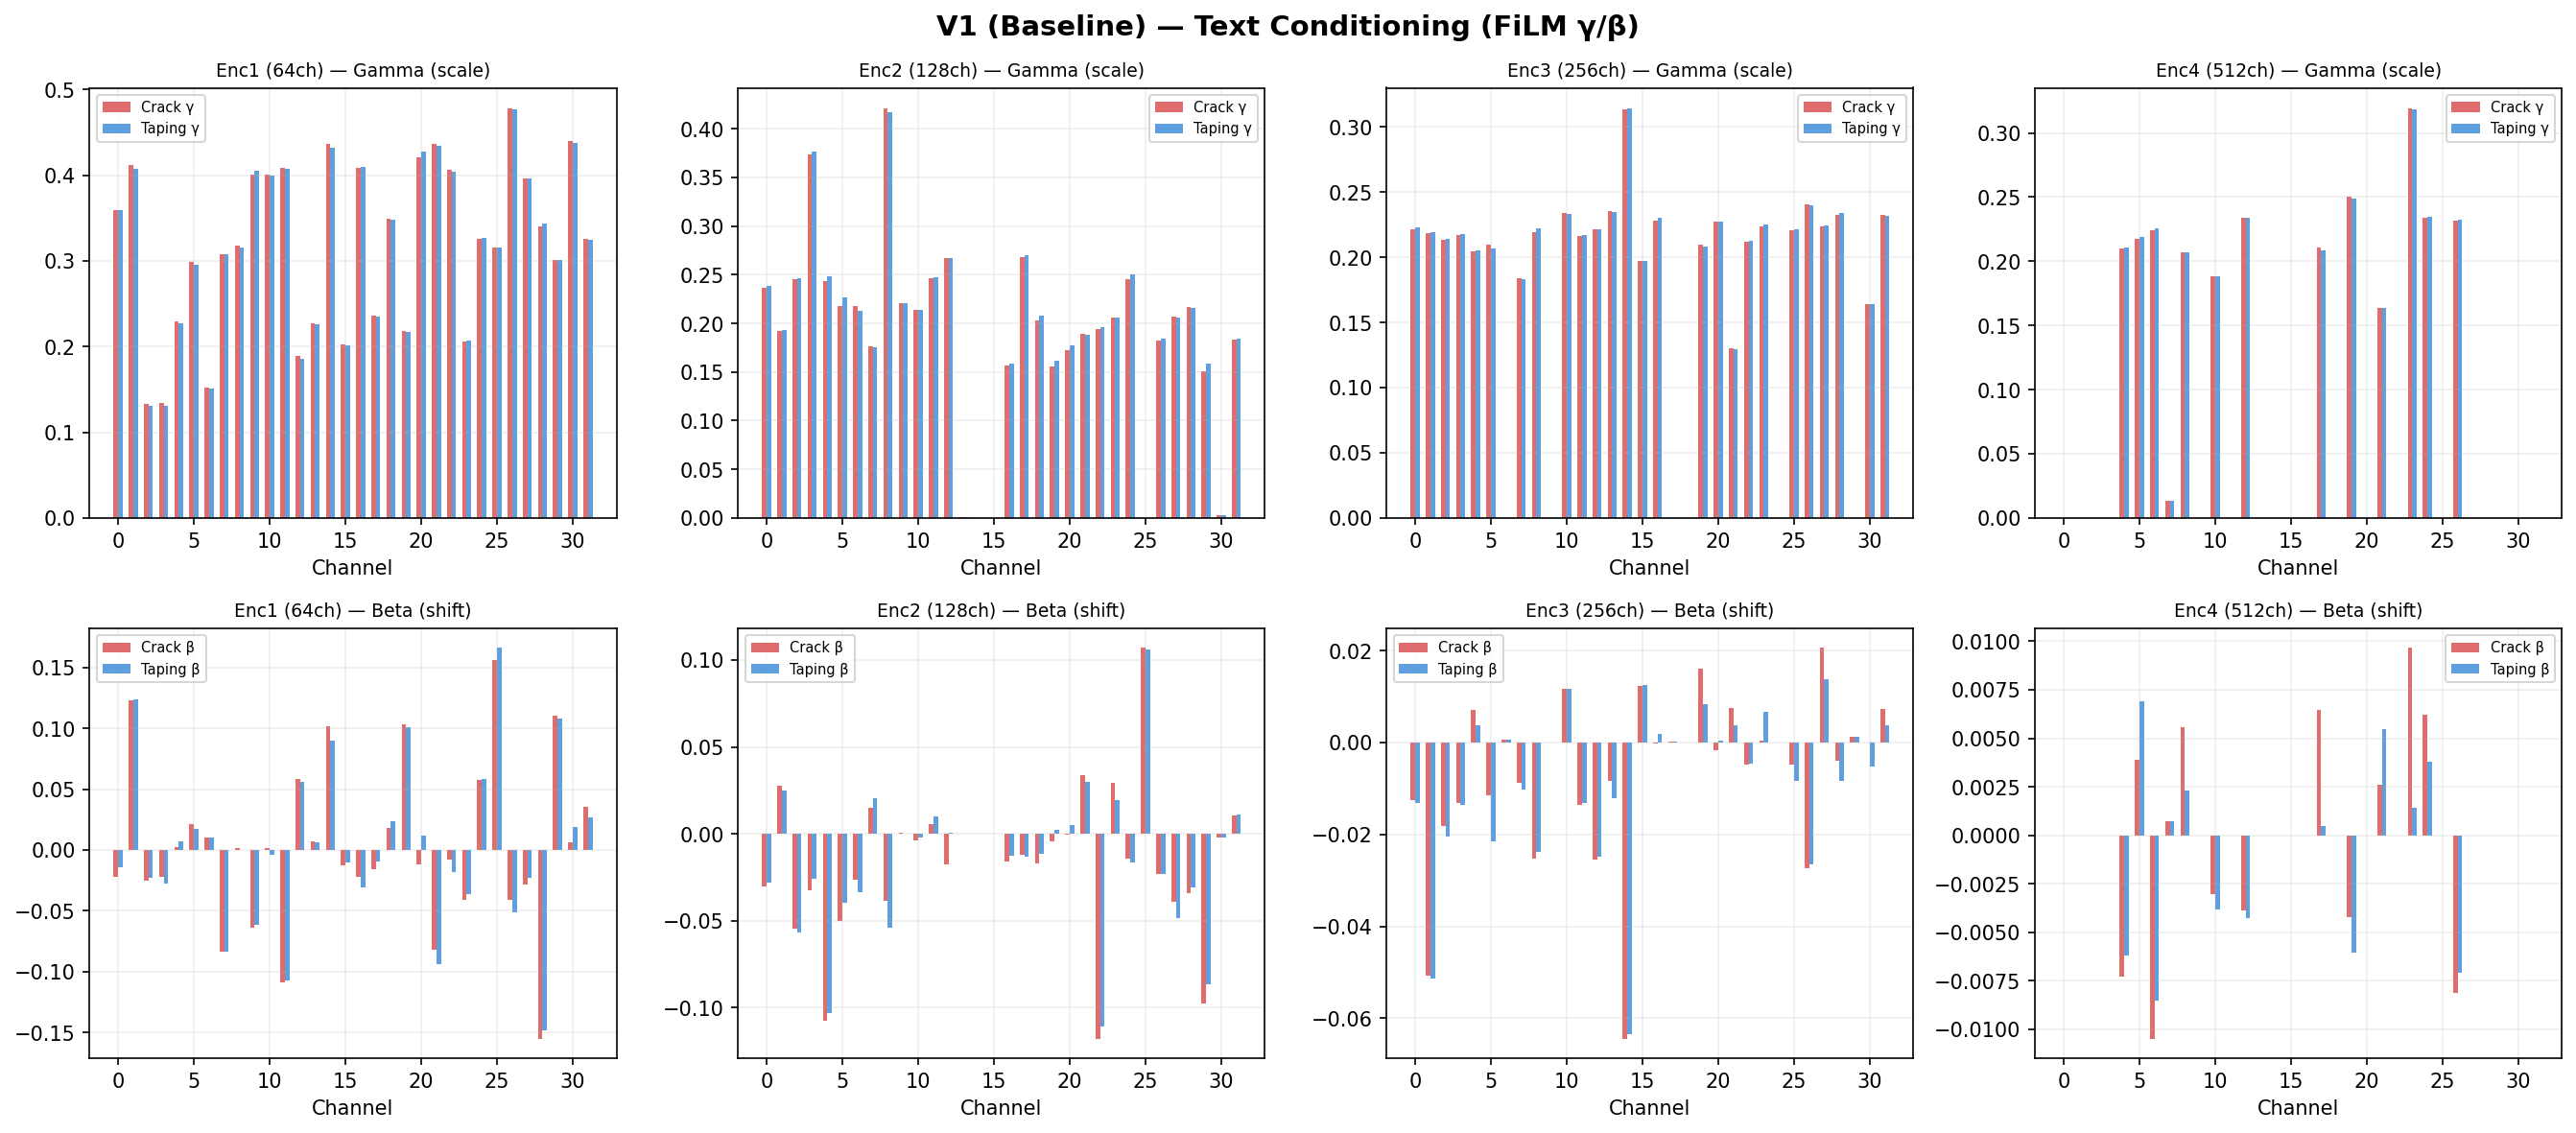
\includegraphics[width=\textwidth]{figures/v1/04_text_conditioning.png}
  \caption{V1 FiLM gamma/beta}
\end{subfigure}
\hfill
\begin{subfigure}{0.48\textwidth}
  
\includegraphics[width=\textwidth]{figures/v2/04_text_conditioning.png}
  \caption{V2 FiLM gamma/beta}
\end{subfigure}
\caption{FiLM modulation parameters for crack vs.\ taping prompts.}
\label{fig:film}
\end{figure}

\subsection{Prompt Validation}

\begin{figure}[H]
\centering
\begin{subfigure}{0.48\textwidth}
  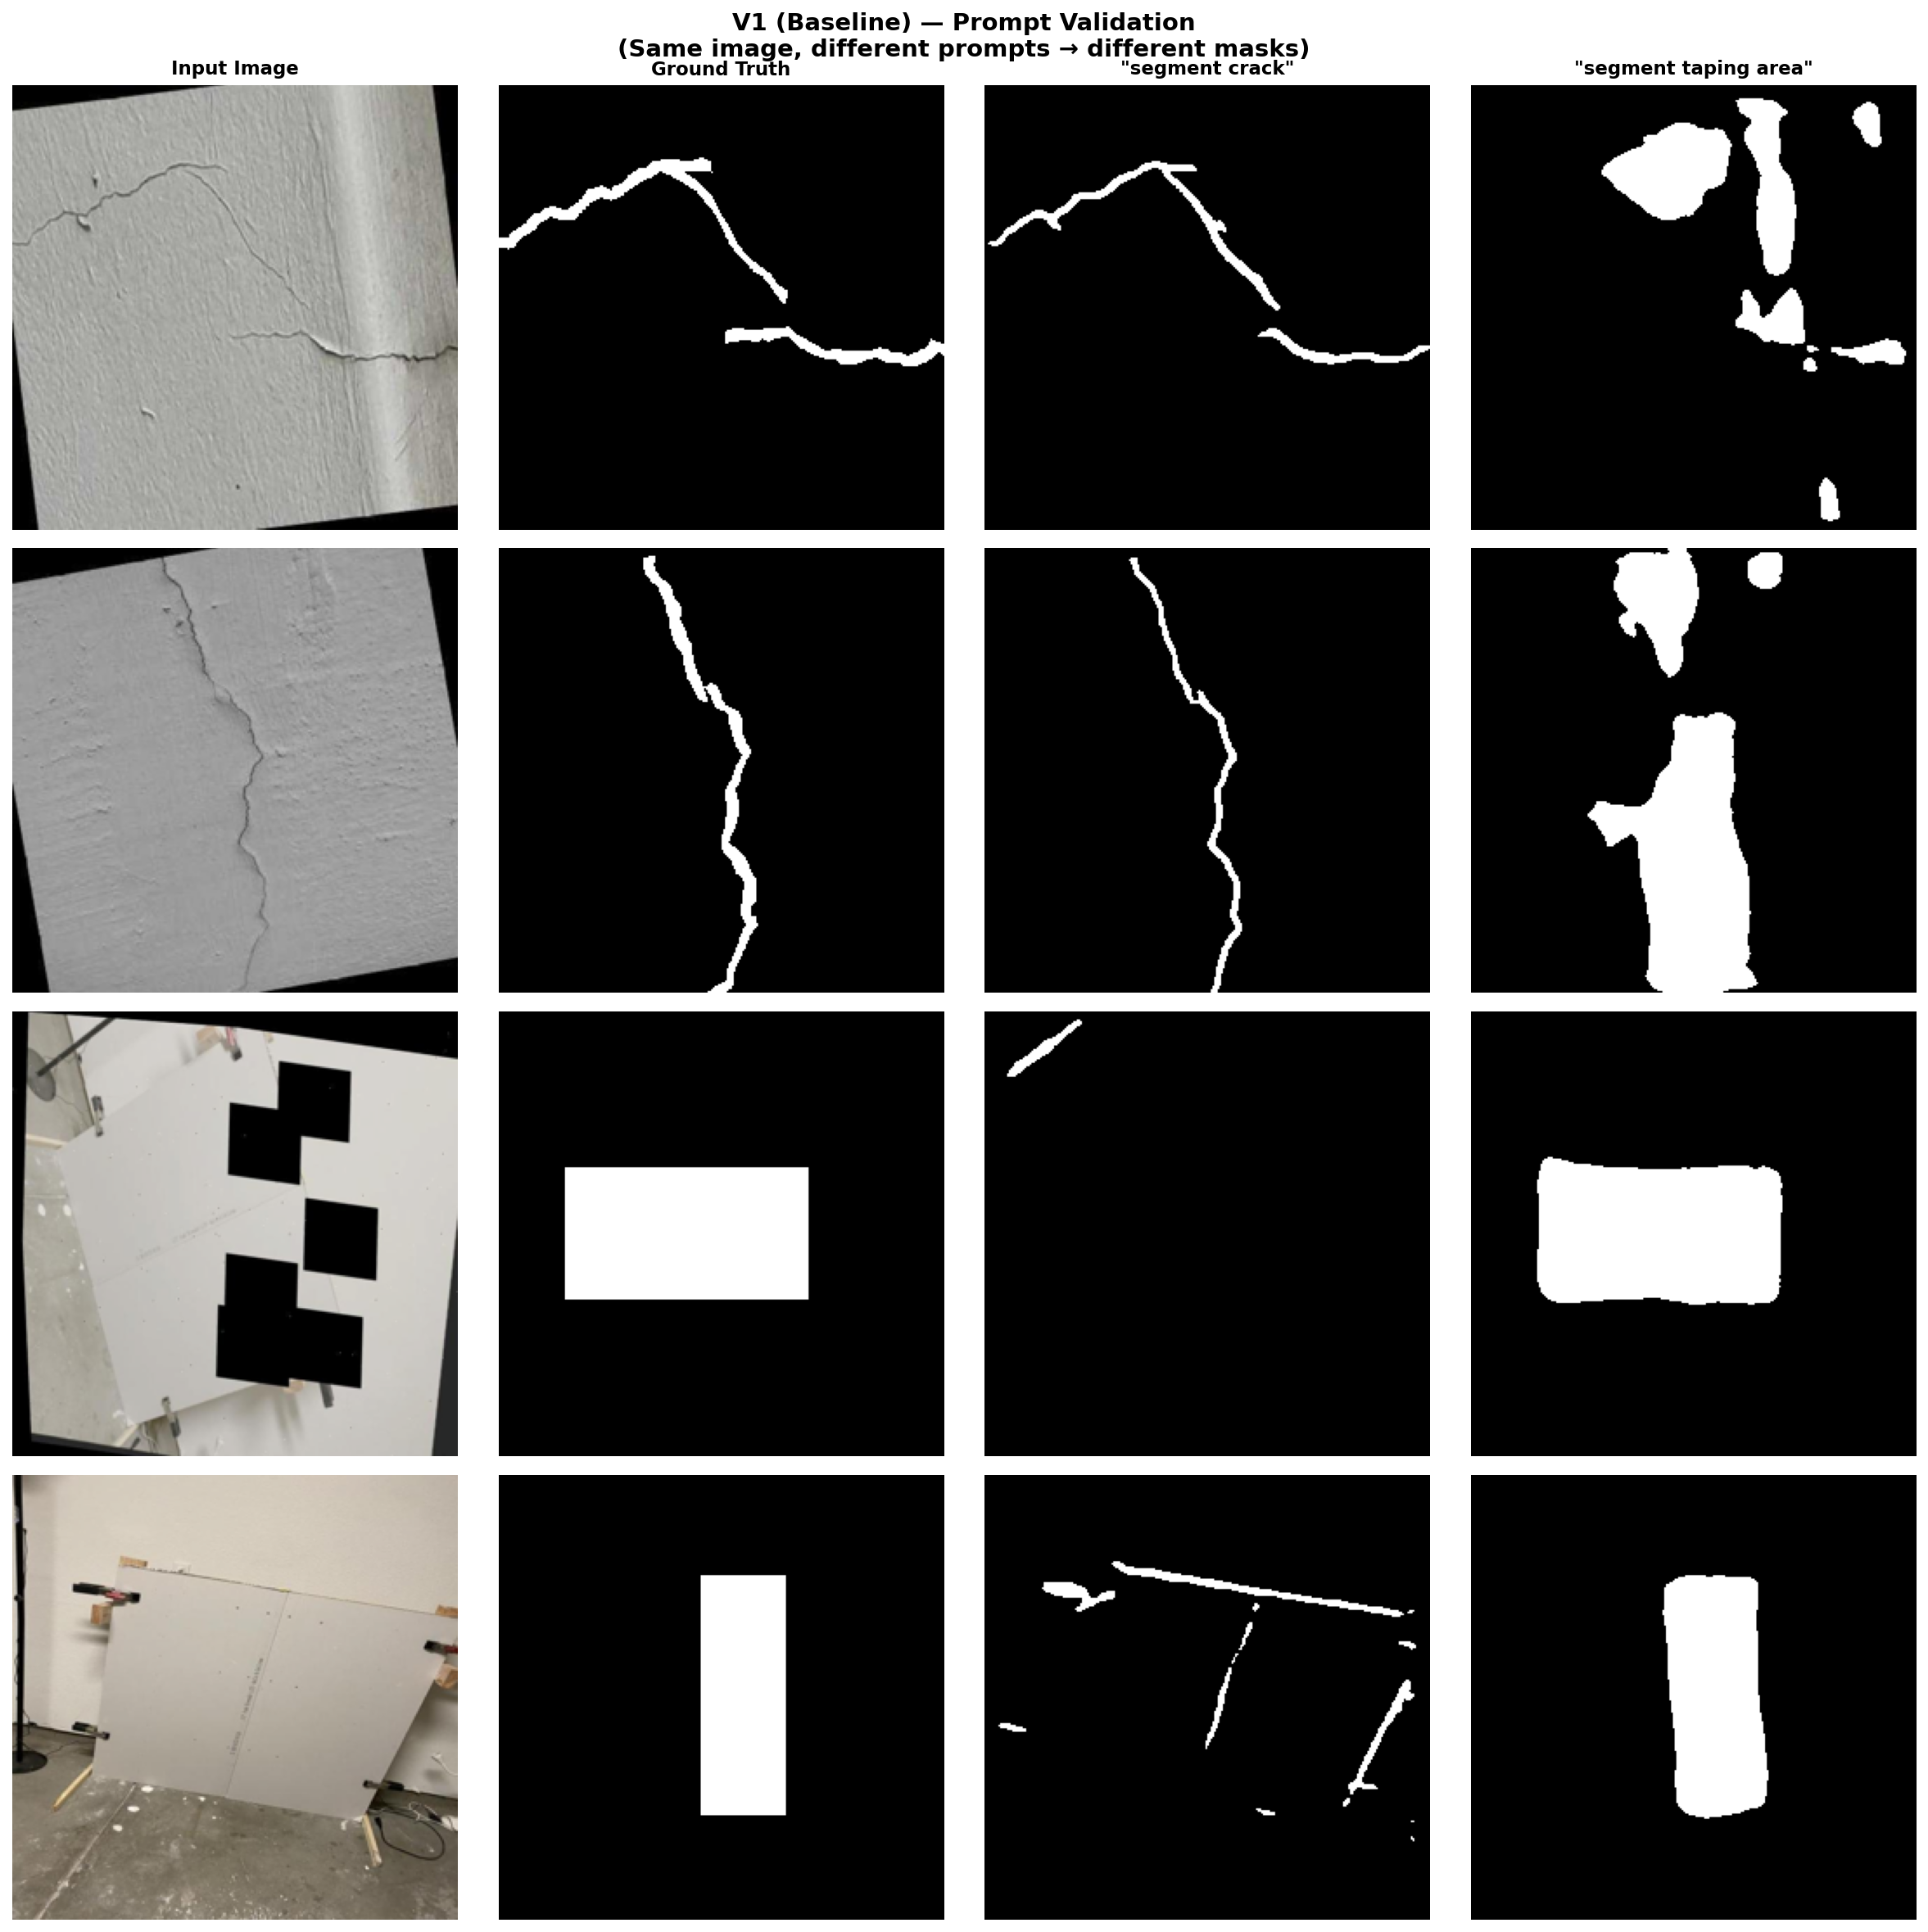
\includegraphics[width=\textwidth]{figures/v1/05_prompt_validation.png}
  \caption{V1 prompt discrimination}
\end{subfigure}
\hfill
\begin{subfigure}{0.48\textwidth}
  
\includegraphics[width=\textwidth]{figures/v2/05_prompt_validation.png}
  \caption{V2 prompt discrimination}
\end{subfigure}
\caption{Same image segmented with \texttt{"segment crack"} vs.\ \texttt{"segment taping area"}.}
\label{fig:prompt}
\end{figure}

% ===== 7. FAILURE NOTES =====================================================
\section{Failure Notes \& Limitations}

\begin{enumerate}[nosep]
  \item \textbf{Thin hairline cracks} ($<$1\% foreground pixels): Even V2 achieves only $\sim$0.44 IoU on very thin cracks because there are so few positive pixels that a single mis-classified pixel shifts the metric drastically.

  \item \textbf{Ambiguous textures}: Mortar lines, shadow edges, and paint imperfections sometimes trigger false positives for the crack prompt, since they share similar gradient patterns.

  \item \textbf{Taping false negatives}: When the taping area is freshly painted and blends with the wall, the model occasionally under-segments, producing fragmented masks.

  \item \textbf{No pretrained backbone}: Training from scratch on $\sim$4.6K images limits the visual features the encoder can learn.  A pretrained ResNet or EfficientNet backbone would almost certainly boost performance, but the assignment required training from scratch.

  \item \textbf{Character-level text encoder}: While functional, it learns only surface-level character patterns rather than true semantic embeddings.  Paraphrased prompts outside the training pool may degrade accuracy.

  \item \textbf{V1$\to$V2 crack gain was modest} (+1.29\,pp IoU): The crack data itself is highly noisy and thin.  My analysis showed that data quality---not model capacity---is the bottleneck.
\end{enumerate}

% ===== 8. RUNTIME & FOOTPRINT ================================================
\section{Runtime \& Footprint}

\begin{table}[H]
\centering
\caption{Runtime and model footprint (V2, NVIDIA L4 24\,GB).}
\begin{tabular}{lr}
\toprule
\textbf{Attribute} & \textbf{Value} \\
\midrule
Total training time (200 epochs) & $\sim$1.5 hours \\
Average inference latency        & 9.70 ms / image \\
Throughput                       & 103 FPS \\
Total parameters                 & 2,752,177 (2.75\,M) \\
Model size (FP32)                & 11.01 MB \\
Model size (FP16)                & 5.5 MB \\
Input resolution                 & 512 $\times$ 512 \\
Batch size (training)            & 16 \\
Mixed precision (AMP)            & Yes \\
GPU memory peak                  & $\sim$8 GB \\
\bottomrule
\end{tabular}
\end{table}

% ===== 9. CONCLUSION =========================================================
\section{Conclusion}

I built PromptSeg-Lite from scratch---a text-prompted segmentation model in under 3M parameters---and iteratively improved it from V1 to V2.  The V2 model achieved mIoU 0.7300 and Dice 0.7796 on a combined drywall taping + surface crack dataset, with real-time inference at 103 FPS.

The iterative V1$\to$V2 process taught me that for this task, higher resolution and a smarter loss function matter more than adding parameters.  The remaining performance bottleneck is data quality, not model capacity: cracks with $<$2\% foreground pixels are inherently hard to segment, regardless of architecture.

The live Streamlit demo and full codebase are available at the links in Section~2.

\vfill
\hrule
\vspace{0.5em}
\small\textit{Generated from the PromptSeg-Lite repository, April 2026.}

\end{document}
